\chapter{Prova de Consentimento}
\label{cap:arquitectura}

O presente capítulo descreve a arquitetura conceptual da solução proposta para a gestão e prova de consentimento digital. Pretende-se apresentar a visão geral do sistema, destacando os principais componentes, a lógica de funcionamento e os mecanismos criptográficos que garantem propriedades fundamentais como autenticidade, integridade, não repúdio, transparência e auditabilidade. Através desta abordagem, é possível assegurar que cada decisão do utilizador é registada de forma verificável e imutável.

\section{Visão Geral da Arquitetura}

É proposto um sistema que define um fluxo de consentimento no qual cada decisão do utilizador é registada, assinada e validada juntamente com o \textit{provedor de serviços}, assegurando que nenhuma das partes pode manipular ou negar a informação posteriormente. Para tal, existem duas entidades principais:

\begin{itemize}
    \item \acrfull{ds}: o utilizador final que interage com a interface web do serviço e fornece o consentimento e que tem uma extensão de navegador à escuta dos eventos do navegador. O \acrshort{ds} é responsável por assinar digitalmente o consentimento antes de o enviar para validação, criando uma prova verificável da sua decisão.
    \item \acrfull{sp}: o \textit{provedor de serviços} que disponibiliza o website com o \acrshort{cmp} à escolha e mantém um servidor para a troca de informação. Isto é, recebe os consentimentos assinados pelo \acrshort{ds}, valida a assinatura do utilizador, assina novamente o consentimento e mantém um registo imutável. Este registo permite auditoria e consulta futura.
\end{itemize}

O fluxo completo do sistema pode ser descrito de forma conceptual:

\begin{enumerate}
    \item O \acrshort{ds} interage com o \textit{banner} de consentimento apresentado pelo \acrshort{cmp} escolhido na interface web fornecida pelo \acrshort{sp}.
    \item A extensão do navegador do \acrshort{ds} captura o evento, prepara o consentimento e assina digitalmente os dados.
    \item O consentimento assinado é enviado ao servidor do \acrshort{sp}, que valida a assinatura do \acrshort{ds} e cria um registo final, incorporando a assinatura do \acrshort{sp}.
    \item O registo resultante é devolvido ao \acrshort{ds}, que pode validar a assinatura do \acrshort{sp}, garantindo que o consentimento foi corretamente registado e não foi alterado.
    \item Ambos, \acrshort{ds} e \acrshort{sp}, mantêm cópias do registo, criando um histórico verificável e auditável. Posteriormente, este pode ser enviado para uma \textit{third-party}, como um \textit{ledger} distribuído.
\end{enumerate}

Este processo pode ser observado de forma mais clara na Figura~\ref{fig:swimlane1}, que ilustra o fluxo completo de interações entre as diferentes entidades do sistema.

Desta forma, o sistema garante quatro propriedades fundamentais. Em primeiro lugar, assegura a \textit{transparência}, uma vez que todos os passos do processo podem ser verificados tanto pelo utilizador como pelo prestador de serviços. Em segundo lugar, garante a \textit{autenticidade} e \textit{integridade} dos consentimentos, através do uso de assinaturas digitais que impedem alterações e confirmam a proveniência das entidades envolvidas. A terceira propriedade é o \textit{não repúdio}, que impede o \acrshort{ds} de negar a sua decisão e o \acrshort{sp} de alegar que não recebeu ou validou o consentimento. Por fim, o sistema promove a \textit{auditabilidade}, mantendo um histórico de consentimentos acessível a ambas as partes, o que permite cumprir os requisitos legais e regulatórios em matéria de proteção de dados.

\section{Componentes}

O sistema é constituído por três componentes principais: a \textit{interface web}, a \textit{extensão do navegador} e o \textit{servidor}.
A interface web representa o ponto de contacto direto com o utilizador e disponibiliza o \textit{banner} de consentimento.
A extensão do navegador atua como intermediário, recebendo os eventos provenientes da interface web feitos pelo utilizador e trata, em segundo plano, do processo de assinatura digital, bem como da autenticação do utilizador através do envio do certificado digital do mesmo.
Por fim, existe um servidor com o qual são trocados os certificados e assinaturas, permitindo que, no final do processo, seja obtido um registo estruturado de consentimento auditável e verificável. Este é responsável por validar as assinaturas recebidas e criar um registo imutável com o consentimento assinado por ambas as partes.

\section{Modelo de confiança}

O processo de recolha e gestão de consentimentos digitais enfrenta vários desafios de confiança.
Em particular, surgem questões relacionadas com a falta de garantias sobre a identidade das entidades envolvidas e a ausência de mecanismos claros de auditoria. 
Estes problemas levantam dúvidas tanto para os \acrshort{ds}, que necessitam de garantias de transparência e controlo sobre as suas decisões, como para os \acrshort{sp}, que precisam de provas fiáveis para demonstrar conformidade regulatória.

Para colmatar estas lacunas, o modelo de confiança proposto assenta em duas camadas principais de proteção: 
\textit{certificados digitais}, que funcionam como método de autenticação das entidades envolvidas, e \textit{assinaturas digitais}, que asseguram a autenticidade, a integridade e o não repúdio das decisões de consentimento. 
Graças a estes mecanismos, cada interação é não só verificável por ambas as partes, como também \textit{auditável}, permitindo a reconstrução fiel do histórico de consentimentos e reforçando a conformidade com requisitos legais como o \acrshort{rgpd}.

\section{Registo do consentimento}

O consentimento do utilizador é preferencialmente um registo estruturado que pode ser interpretado e processado de forma padronizada. Este registo deve ser interoperável, auditável e verificável, permitindo que diferentes sistemas o leiam e validem sem ambiguidade.

Para garantir estas propriedades, o consentimento é assinado digitalmente tanto pelo utilizador como pela entidade que o recebe. A troca de certificados entre as partes possibilita a verificação mútua das assinaturas, reforçando a confiança no processo. O objecto resultante agrega informação relevante sobre as decisões do utilizador, bem como metadados necessários à validação, mantendo a integridade e autenticidade do consentimento.

A ausência de cifragem no registo de consentimento simplifica o processo de verificação e auditoria, mas aumenta o risco de exposição de informação pessoal. Mesmo que o registo não contenha dados diretamente identificáveis, como o nome ou o e-mail, pode incluir identificadores indiretos, por exemplo, identificadores únicos, que podem permitir reconhecer ou reidentificar o utilizador. Para reduzir este risco e garantir conformidade com o princípio da confidencialidade previsto nas legislações, recomenda-se a aplicação de técnicas complementares de pseudonimização ou cifragem seletiva, de modo a equilibrar a transparência com a proteção da privacidade do utilizador.

\section{Interação Entre Componentes}

A figura~\ref{fig:swimlane1} ilustra o fluxo completo de troca de mensagens e assinaturas durante o processo de consentimento. O sistema envolve três componentes principais: o \textit{cliente}, que inclui a extensão do navegador para capturar e assinar digitalmente os consentimentos; a \textit{interface web} do \textit{prestador de serviços}, que apresenta o \textit{banner} de consentimento; e o \textit{servidor}, responsável por validar e assinar os registos de consentimento.

Quando o utilizador acede ao website, a interface web apresenta o \textit{banner} de consentimento e juntamente envia o certificado do servidor. O utilizador preenche o \textit{banner} e, através da extensão do navegador, assina digitalmente o consentimento utilizando a sua chave privada. A extensão prepara então o objeto final do consentimento, que inclui a assinatura do utilizador, e envia-o para o servidor juntamente com o certificado do cliente.

O servidor valida a assinatura do utilizador e o respetivo certificado, gera a sua própria assinatura digital sobre o consentimento e cria um registo final que agrega ambas as assinaturas. Este registo é devolvido ao cliente, que valida a assinatura do servidor e mantém uma cópia do consentimento de forma verificável.

Desta forma, o fluxo garante que, tanto o cliente como o servidor, dispõem de provas verificáveis e mutuamente validadas do consentimento, assegurando transparência, integridade e auditabilidade ao longo de todo o processo.

\begin{figure}[h]
\begin{center}
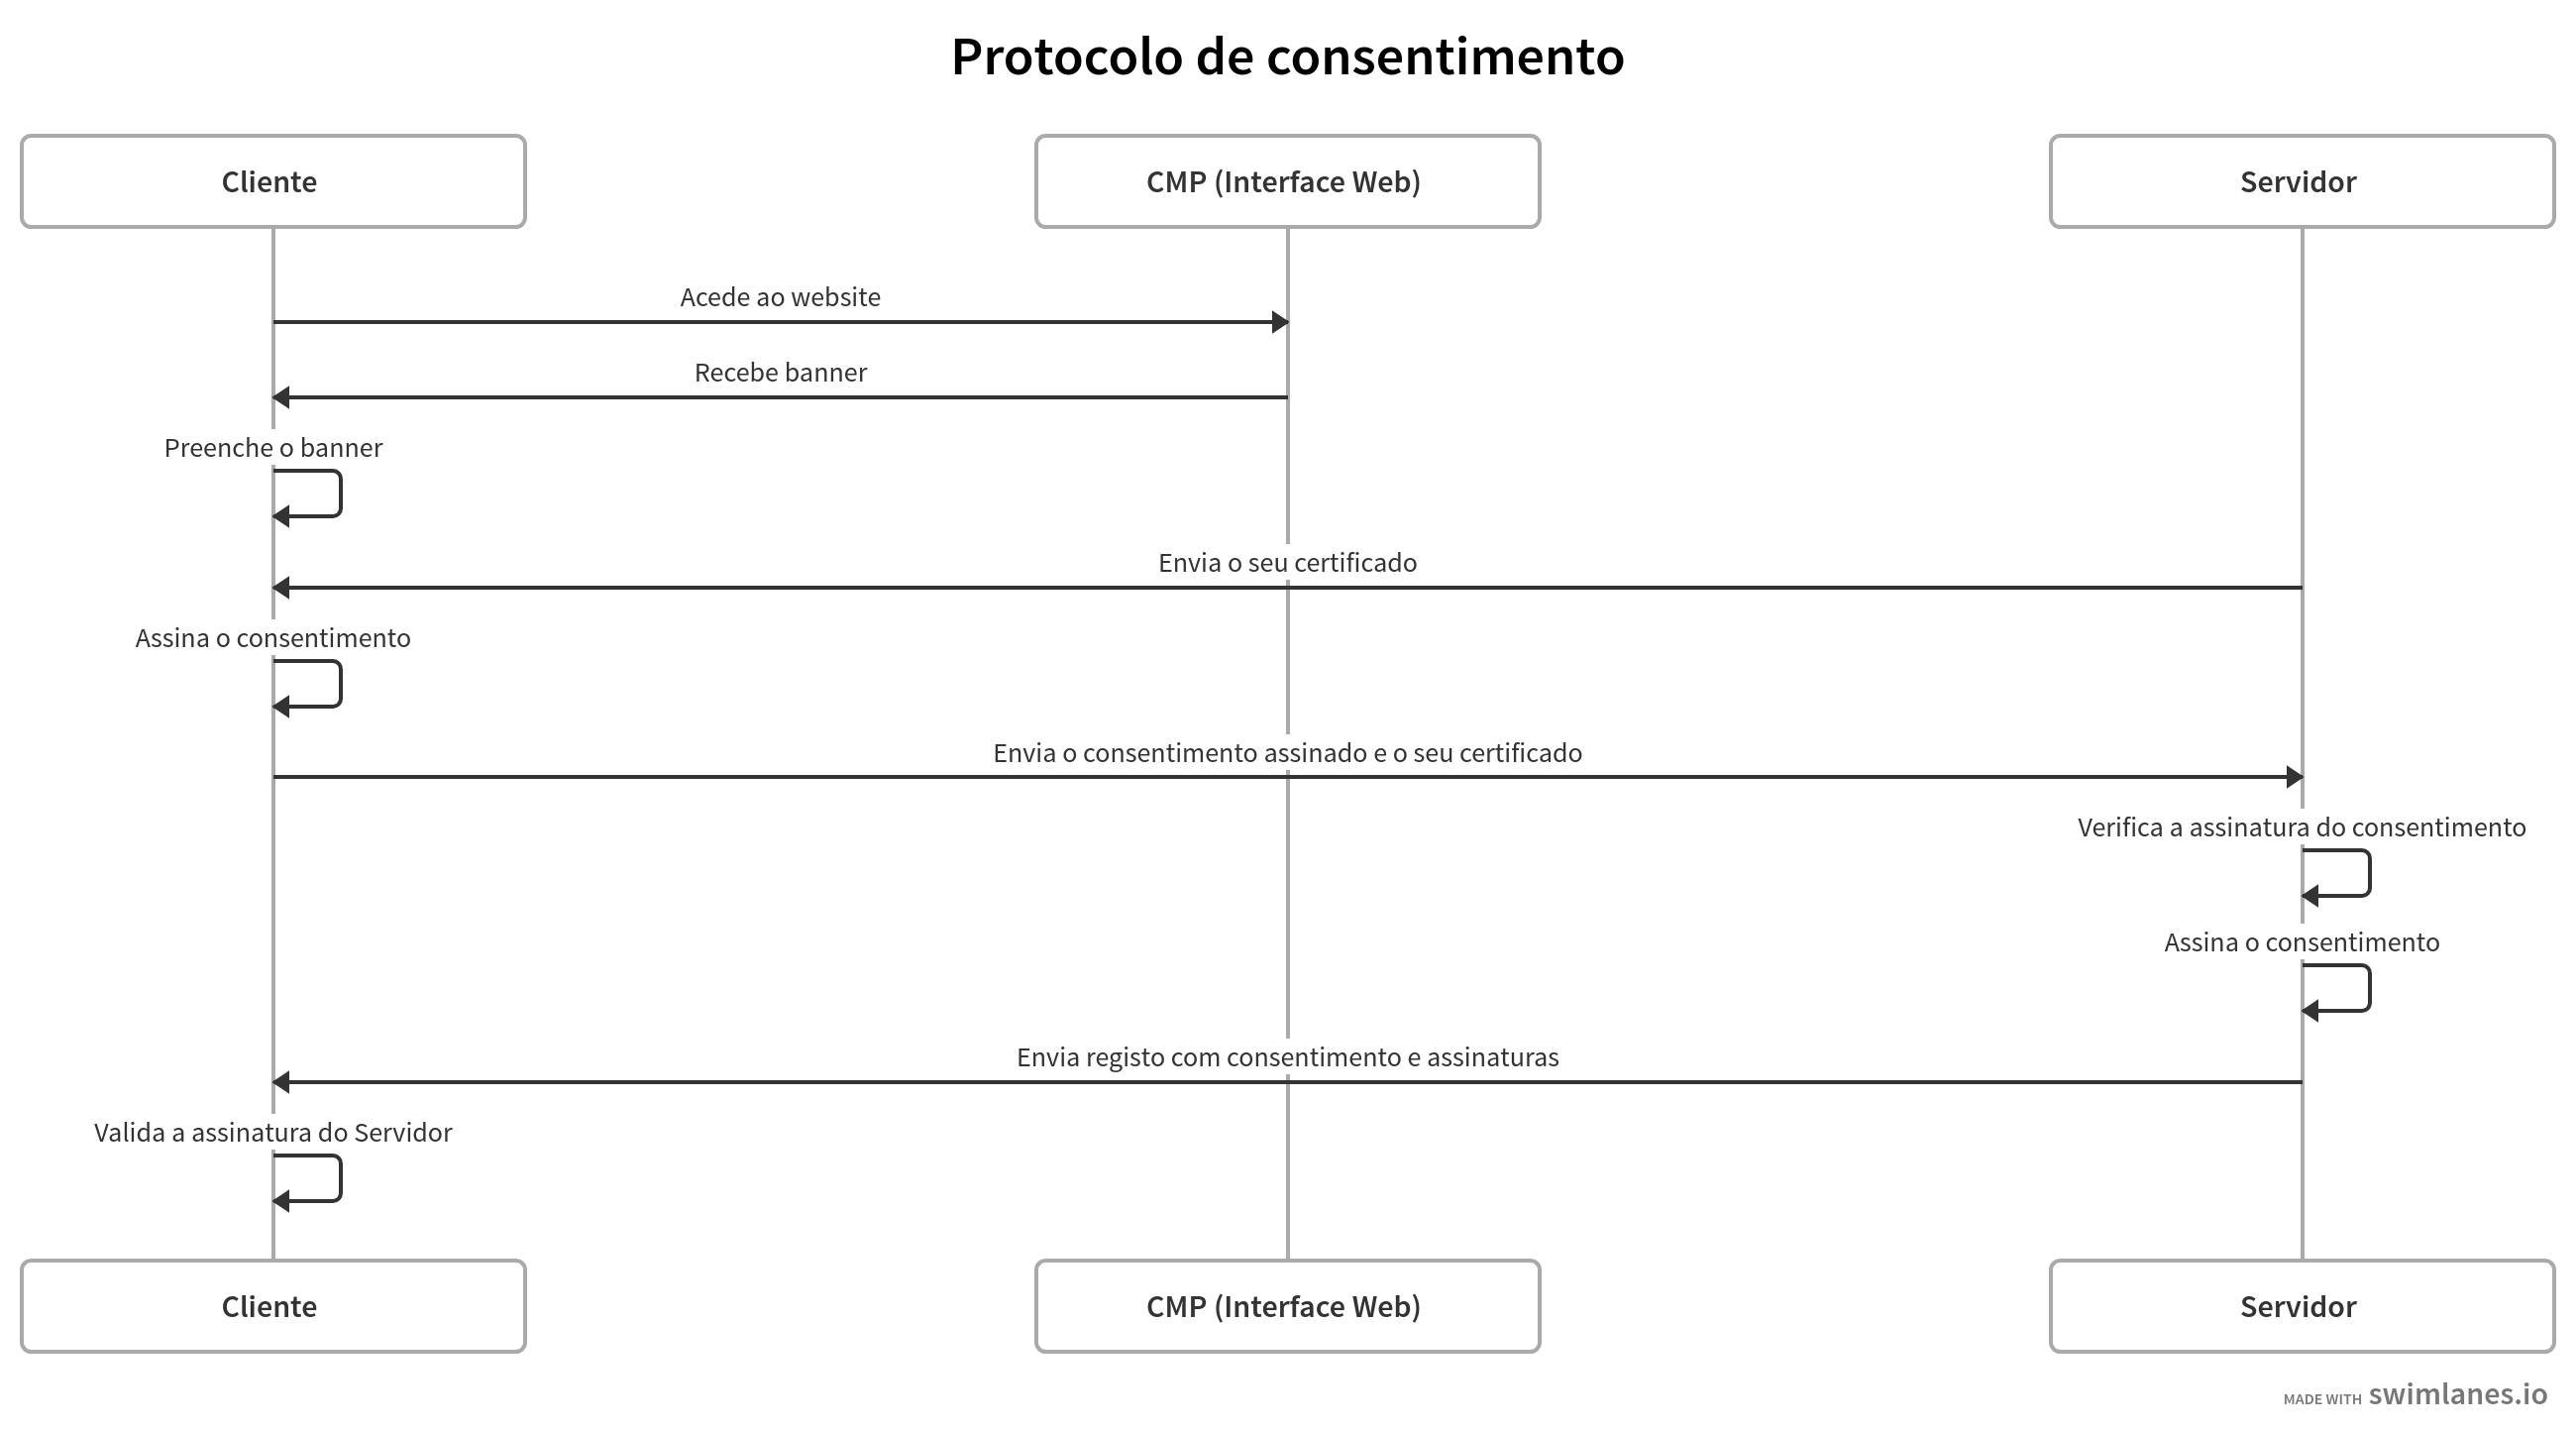
\includegraphics[width=1\textwidth]{images/swimlanes.png}
\end{center}
\caption{Diagrama do protocolo de \textit{Prova de Consentimento}.}
\label{fig:swimlane1}
\end{figure}

\newpage

A estratégia proposta assenta numa abordagem de assinaturas digitais, na qual o cliente e servidor participam ativamente na criação de um registo de consentimento verificável e imutável. Esta abordagem garante quatro propriedades fundamentais: \textit{transparência}, na medida em que todos os passos podem ser verificados; \textit{descentralização}, dado que nenhuma das partes detém controlo unilateral; \textit{não-repúdio}, assegurando que os consentimentos prestados não podem ser posteriormente negados; e \textit{auditabilidade}, uma vez que o histórico completo permanece acessível tanto localmente, junto de cada entidade participante, como opcionalmente através de um serviço de terceiros responsável pela verificação ou conservação dos registos.

\section{Benefícios}

A \textit{Prova de Consentimento} proposta apresenta benefícios distintos para os diferentes intervenientes.
Do ponto de vista do utilizador, este tem a possibilidade de verificar a integridade dos registos, garantindo que não foram alvo de manipulação. Dispõe ainda de recursos que lhe conferem autonomia para obter uma prova dos seus consentimentos, que se tornariam especialmente relevantes na verificação do incumprimento dos mesmos.

Para as organizações, a arquitetura disponibiliza provas fiáveis de consentimentos válidos, que podem ser utilizadas em auditorias ou processos de verificação de conformidade.
Deste modo, contribui para a redução dos riscos associados ao incumprimento das regulamentações em vigor, promovendo maior confiança e segurança jurídica no tratamento de dados pessoais.

\section{Síntese do capítulo}

Neste capítulo foi apresentada a arquitetura conceptual da solução de \textit{Prova de Consentimento}, detalhando os principais componentes, a lógica de funcionamento e os mecanismos criptográficos, como certificados digitais e assinaturas digitais. Através da Prova de Conceito, demonstrou-se a viabilidade do modelo conceptual, validando a autenticidade, integridade, não repúdio, transparência e auditabilidade dos registos de consentimento num ambiente simplificado, sem recorrer ainda a uma implementação completa.

O capítulo seguinte descreve a implementação prática desta arquitetura, materializada num protótipo funcional que integra os princípios validados na Prova de Conceito. Nesta fase, são exploradas tecnologias reais e fluxos completos, permitindo avaliar o desempenho, a interoperabilidade e a experiência de utilização, evidenciando os benefícios e limitações do sistema face às limitações identificadas no trabalho relacionado (\ref{cap:relacionado}).
